\documentclass[a5paper,final]{memoir}
%\usepackage[a5paper]{geometry}
\usepackage{mathpazo}
%\usepackage{newpxmath}
\usepackage[final]{graphicx}
\usepackage[final]{listings}
\usepackage[utf8]{inputenc}
\usepackage[english]{babel}
\usepackage[T1]{fontenc}
\usepackage{imakeidx}
%\usepackage{marginnote}
\usepackage[table]{xcolor}
\usepackage{caption}
\usepackage{float}
  \floatstyle{boxed}
  \newfloat{pulledtext}{tbp}{pulledtext}
\lstset{
  showstringspaces=false,
  language=tcl,
  frame=lines,
  aboveskip=\bigskipamount,
  belowskip=\bigskipamount,
  numbers=left,
  numberstyle=\tiny,
  firstnumber=last,
  basicstyle=\footnotesize\ttfamily,
}
%\renewcommand{\thesection}{\arabic{section}}
\title{Into the Interpreter\\with ConsTcl}
\author{Peter Lewerin}
\date{\today}
\makeatletter
\def\@makechapterhead#1{%
  \vspace*{50\p@}%
    {\parindent \z@ \raggedright \normalfont
      \ifnum \c@secnumdepth >\m@ne
        %\if@mainmatter
          %\huge\bfseries \@chapapp\space \thechapter
          \Huge\bfseries \thechapter.\space%
          %\par\nobreak
          %\vskip 20\p@
        %\fi
      \fi
      \interlinepenalty\@M
      \Huge \bfseries #1\par\nobreak
      \vskip 40\p@
   }}
\makeatother
\makeindex[intoc]
\counterwithout{footnote}{chapter}
\setcounter{secnumdepth}{1}
\hyphenation{Cons-Tcl}
\hyphenation{ins-tan-ce}
\hyphenation{na-me-spa-ce}
\hyphenation{need-ed}
\hyphenation{back-slash}
\hyphenation{ta-kes}
\hyphenation{look-up}
\hyphenation{bool-ean}
\hyphenation{search-es}
\hyphenation{expres-sion}

\begin{document}

\frontmatter
\pagestyle{empty}
\begin{flushright}
{Into the Interpreter}
\end{flushright}
\cleardoublepage

\begin{center}
{\Huge\sffamily\thetitle}

\vspace{0.7in}
\theauthor

\end{center}
\clearpage

\begin{center}
{\small

Automatiserad teknik vilken används för att analysera text och data i digital
form i syfte att generera information, enligt 15a, 15b och 15c \S\S\ 
upphovsrättslagen (text- och datautvinning), är förbjuden.

\textcopyright\ 2025 Peter J Lewerin\\
($\phi$) Funktion förlag, Tidaholm
}
\end{center}
\clearpage

\pagestyle{plain}

\renewcommand*{\contentsname}{Short contents}
\setcounter{tocdepth}{0}% chapters and above
\tableofcontents
\clearpage
\renewcommand*{\contentsname}{Contents}
\setcounter{tocdepth}{2}% subsections and above
\tableofcontents

\addcontentsline{toc}{section}{Introduction}
\chapter*{Introduction}
\label{introduction}
\addcontentsline{toc}{section}{To run the software}
\section*{To run the software}
\label{to-run-the-software}


First things first. To run the software, source the file \textbf{constcl.tcl}
(with \textbf{schemebase.scm} in the directory) in a Tcl console (I use
\textbf{tkcon}) and use the command \textbf{repl} for a primitive command
dialog. Source \textbf{all.tcl} to run the test suite (you need
\textbf{constcl.test} for that). The files can be found on
GitHub/ConsTcl\footnote{See \texttt{https://github.com/hoodiecrow/ConsTcl}}.

The following license holds for the software, not the book:

\subsection{MIT License}
\label{mit-license}
\index{MIT License}

Copyright (c) 2025 Peter Lewerin

Permission is hereby granted, free of charge, to any person obtaining a copy
of this software and associated documentation files (the "Software"), to deal
in the Software without restriction, including without limitation the rights
to use, copy, modify, merge, publish, distribute, sublicense, and/or sell
copies of the Software, and to permit persons to whom the Software is
furnished to do so, subject to the following conditions:

The above copyright notice and this permission notice shall be included in all
copies or substantial portions of the Software.

THE SOFTWARE IS PROVIDED "AS IS", WITHOUT WARRANTY OF ANY KIND, EXPRESS OR
IMPLIED, INCLUDING BUT NOT LIMITED TO THE WARRANTIES OF MERCHANTABILITY,
FITNESS FOR A PARTICULAR PURPOSE AND NONINFRINGEMENT\@. IN NO EVENT SHALL THE
AUTHORS OR COPYRIGHT HOLDERS BE LIABLE FOR ANY CLAIM, DAMAGES OR OTHER
LIABILITY, WHETHER IN AN ACTION OF CONTRACT, TORT OR OTHERWISE, ARISING FROM,
OUT OF OR IN CONNECTION WITH THE SOFTWARE OR THE USE OR OTHER DEALINGS IN THE
SOFTWARE.

The software is pretty much harmless, but there is a potential danger if anyone
were to use it to write and run Scheme code that uses the output functions and
in the process were careless enough to let the code overwrite existing files. I
have put safeguards in the output functions that need to be removed before they
work.

The software works for me, but there might still be problems that I haven't
noticed. Contact me at

\indent \texttt{constcl1000@gmail.com}

with any queries or error reports. I intend to keep updating the software to
include bug fixes and interesting additions, within reason.

\addcontentsline{toc}{section}{Background}
\section*{Background}
\label{background}

It all started with Peter Norvig's\index{Norvig, Peter} Lisp emulator
Lispy\footnote{See \texttt{https://norvig.com/lispy.html}}. In January 2025 I
was inspired to port it to Tcl. The result was Thtcl\footnote{See
\texttt{https://github.com/hoodiecrow/thtcl}}. It had the same features and
limitations as Lispy, plus a couple of limitations that were due to
shortcomings of Tcl, and I came out of the experience feeling a bit
dissatisfied. In the latter part of January I embarked on a new project,
ConsTcl, a true Lisp interpreter. In Tcl.

\subsection{About Lisp}
\label{about-lisp}

ConsTcl is a \emph{Lisp interpreter}, specifically a \emph{Scheme interpreter}.
Lisp is a family of programming languages that share the same basic form, and
Scheme is one of those languages. Where some other languages use braces to
structure code, and Python uses indents, Lisp instead uses parentheses. This
Python snippet:

\begin{verbatim}
x = 1
if x == 1:
    print("x is 1.")
\end{verbatim}

\noindent looks like this in Scheme:

\begin{verbatim}
(let ((x 1))
  (if (= x 1)
    (write "x is 1.")))
\end{verbatim}

In Lisp, everything is either an \emph{atom}, an indivisible value, like
\texttt{x} and \texttt{1} (and e.g. \texttt{let} and \texttt{write} too) or
else it is a \emph{list expression}, starting and ending with parentheses and
having an operator at the front of the list, with the rest of the parts being
operands. If the operator is a keyword like \texttt{let} or \texttt{if}, then
the expression is a \emph{special form}. If not, like \texttt{=} or
\texttt{write}, then it's a \emph{function call}.

A full description of Lisp is beyond the scope of this introduction, but Lisp
will be explained from the inside out in the rest of this book. If you want to
learn Scheme right away, there are good tutorials in
different\footnote{See \texttt{https://docs.scheme.org/schintro/}}
places\footnote{See \texttt{https://www.scheme.com/tspl4/}} on the
web\footnote{See
\texttt{https://files.spritely.institute/papers/scheme-primer.html}}.

\subsection{About ConsTcl}
\label{about-constcl}

Compared to Lispy/Thtcl, ConsTcl has, (quote from Lispy), ``comments, quote and
quasiquote notation, \# literals, the derived expression types (such as cond,
derived from if, or let, derived from lambda), and dotted list notation.''
Again compared to Lispy/Thtcl, ConsTcl has the data types, quote, ``strings,
characters, booleans, ports, vectors.'' And pairs and procedures too. The
number of missing primitive procedures is in the tens, not the 100s. 

The completeness comes with a price: due to the sheer number of calls for each
action, ConsTcl is is fairly slow. On my cheap computer, the following code
(which calculates the factorial of 100) takes 0.04 seconds to run. That is thirteen
times slower than Lispy assuming that Norvig's computer is as slow as mine,
which is unlikely.

\begin{verbatim}
time {pe "(fact 100)"} 10
\end{verbatim}

ConsTcl is of course still limited. It doesn't come close to having call/cc or
tail recursion. It doesn't have exact/inexact numbers, or most of the numerical
tower. There is no memory management. Error reporting is spotty, and there is no
error recovery.

\subsection{About the book}
\label{about-the-book}


I like writing documentation, and occasionally I'm good at it. I like to
annotate the source code with bits of documentation, which I then extract and
put together using tools like \texttt{awk}. It looks like this:

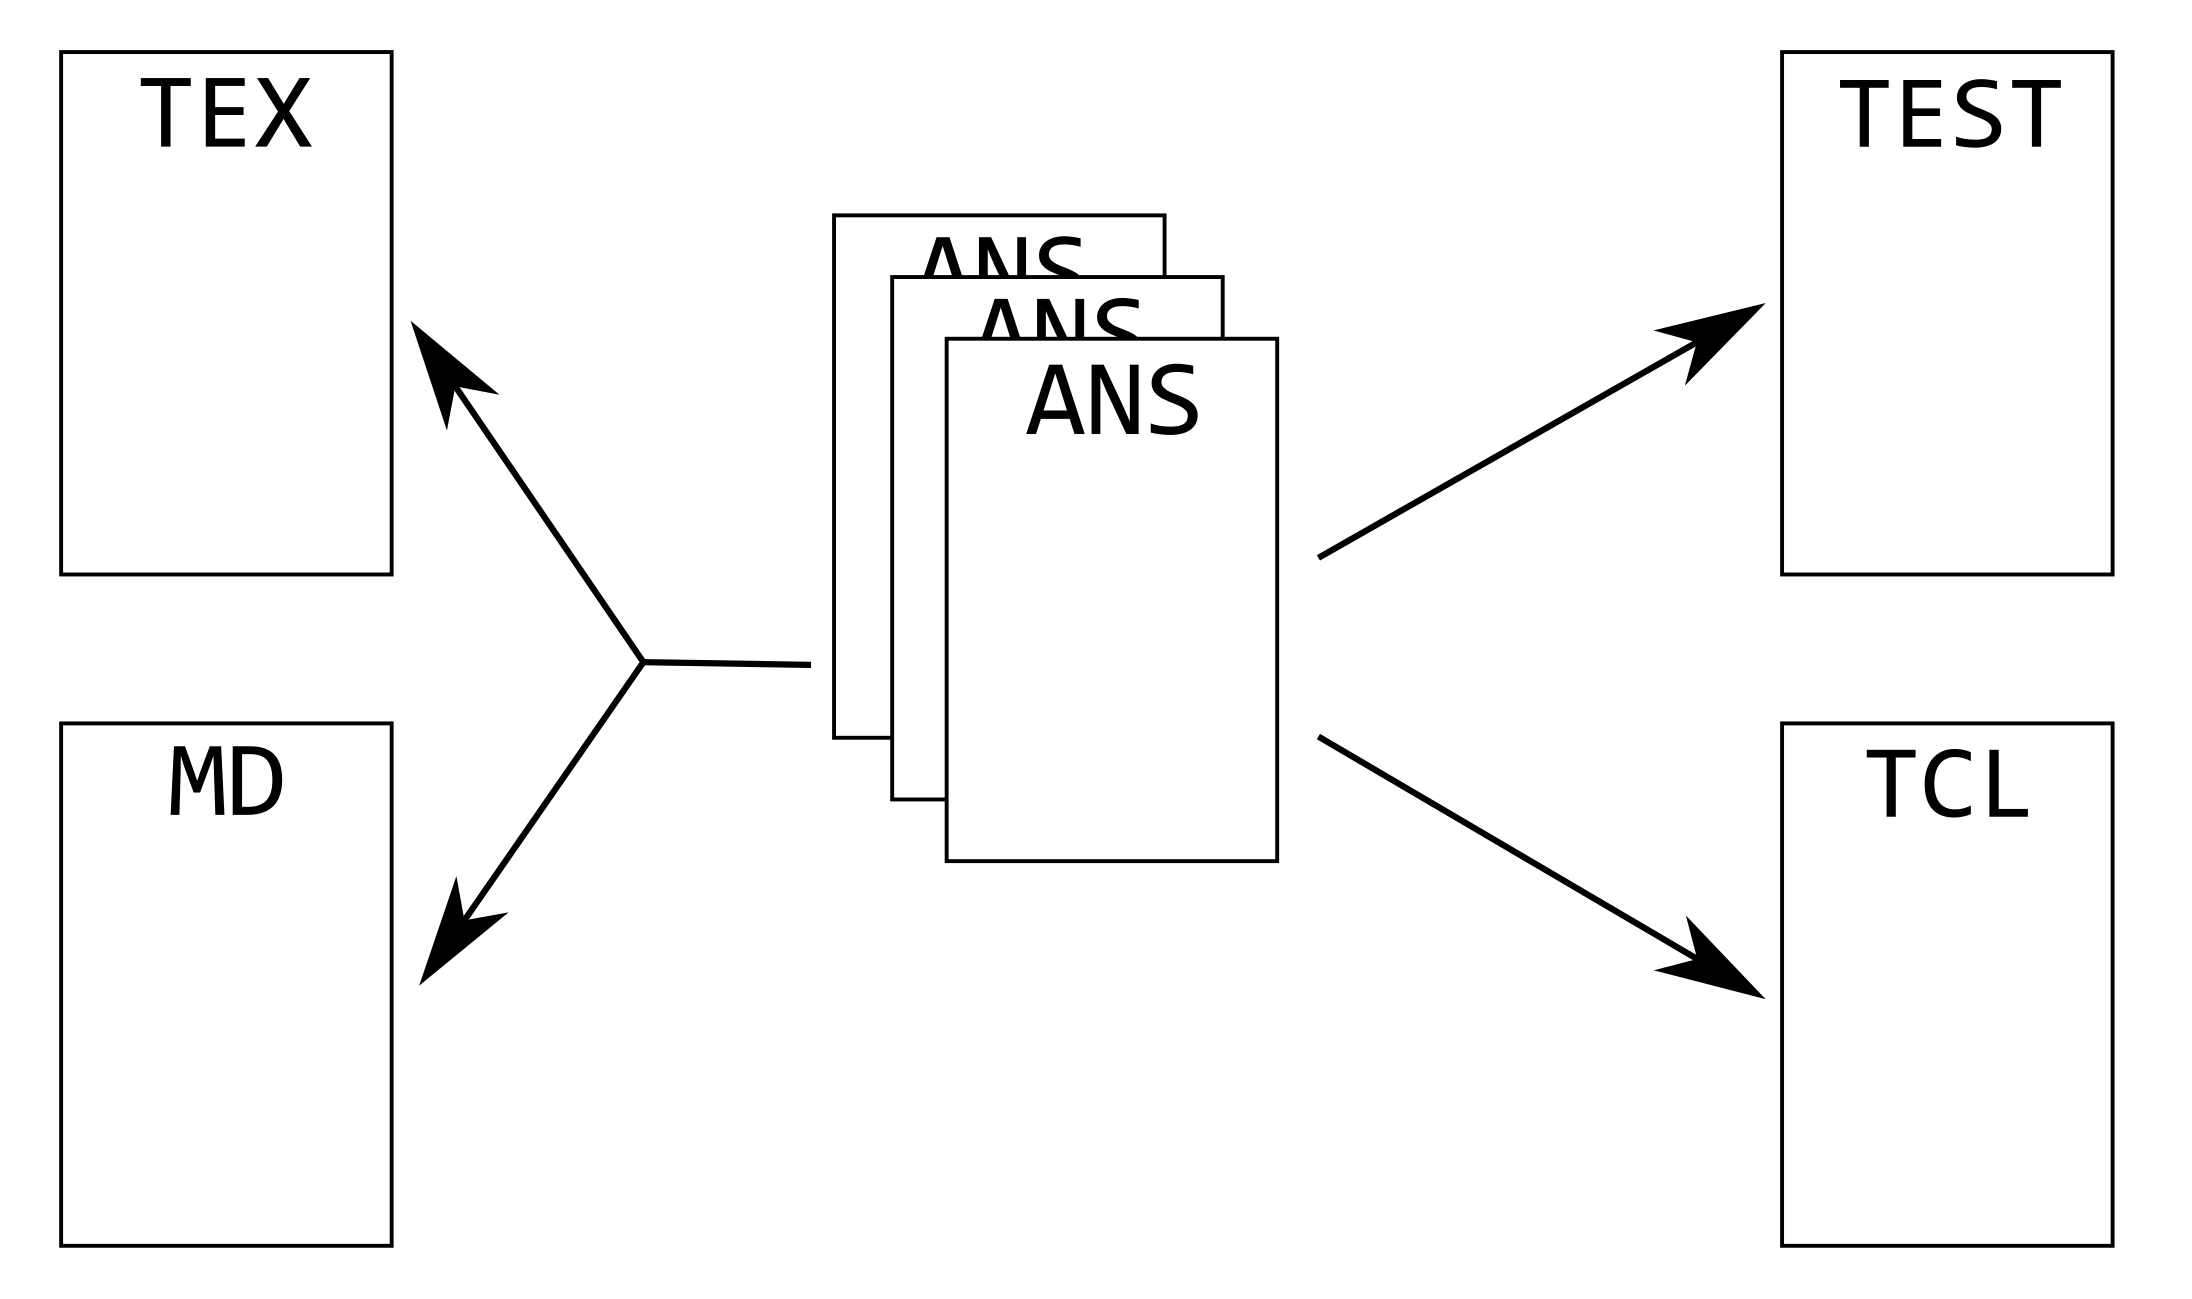
\includegraphics{images/document.png}

In the middle are a bunch of \texttt{.ans} files (ANnotated Source). These are
written with Vim. From the TT tags of those, I extract a \texttt{.test} file.
From the CB tags I extract \texttt{.tcl} source (or Scheme or C source, as the
case might be). From all the tags except TT I extract formatted documentation
in Markdown and \LaTeX{} format. All these extractions are automated using
\texttt{make}.  Figures are made with Inkscape.  I create a PDF document from
the \LaTeX{} source using TeXworks. On finishing up ConsTcl, it struck me that
the documentation for this piece of software was fit for a book.

ConsTcl is at least 97\% my own work, but I have ported one part (see page
\pageref{resolving-local-defines}) from ``Scheme 9 from Empty
Space''\footnote{See \texttt{https://t3x.org/s9book/index.html}}\index{Scheme 9
from Empty Space}\index{S9fES} by Nils M Holm\index{Holm, Nils M}, a Lisp
interpreter written in C and commented in a similar manner to this book.

One source which I spent a lot more time with was R5RS\footnote{Revised${}^{5}$
Report on the Algorithmic Language Scheme, Scheme's standardization document},
\emph{the} authoritative manual on Scheme. It says nothing about the
implementation of the interpreter, but a lot on what features the language has
and how they are supposed to work.

Another source of guidance and inspiration was ``Lisp in Small Pieces'' by
Christian Queinnec. Yet another source was ``An Introduction to Scheme and its
Implementation''\footnote{See \texttt{https://docs.scheme.org/schintro/}}.

\subsection{About the program listings}
\label{about-the-program-listings}

I have tried to write clear, readable code, but the page format forces me to
shorten lines. I have used two-space indents instead of four-space, a smaller
font, and broken off long lines with a \textbackslash\  at the end of the first
line (a so-called `tucked-in tail'). Neither of these measures improve
readability, but the alternative is overwriting the margins. Not all broken
lines have the \textbackslash: some are broken inside a
\texttt{\{}\ldots\texttt{\}} block, and some right after a \texttt{^^5b}.

\subsection{About me}
\label{about-me}

I'm a 60 year old former system manager who has been active in programming
since 1979. Currently, and for some time, my language of choice is the
rather marginal Tcl\footnote{See \texttt{https://www.tcl-lang.org/}} (it's not
even in the 100 most used languages). Tcl suits me, and there are things that
one can do in Tcl that one can't easily do in other languages. Lisp is a
runner-up in my affections, a language that fascinates me but doesn't fit my
brain very well (though I have written one large piece of software in AutoLisp,
a CAD subsystem for designing drilling boxes).

In addition to my terms as programmer and system manager, I have worked as a
teacher (teaching C/C++ in upper secondary school) and for a short while I
wrote manuals for the department for information technology at
the University of Skövde. I've also been active writing answers at
question-and-answer sites on the web, mainly Stack Overflow.

\subsection{About time}
\label{about-time}

I'd like to thank

\begin{itemize}
\item my children and their lifemates for being awesome.

\item my mother and my ex-wife for supporting the printing of the book financially.

\item my sister and brother-in-law for being supportive.
\end{itemize}

\vspace{1in}\noindent And now let's journey into the Interpreter.

\mainmatter
\pagestyle{headings}

